\documentclass[11pt]{article}
\usepackage[utf8]{inputenc}
\usepackage{graphicx}
\usepackage{amssymb,amsmath,amsthm,amsfonts}
\usepackage{amsfonts}
\usepackage[usenames,dvipsnames]{color}
% \usepackage{kpfonts}
\usepackage{algorithm}
\usepackage[noend]{algorithmic}
\usepackage[square, comma, numbers,sort&compress]{natbib}
\usepackage{cleveref}
\usepackage{blindtext}
\usepackage{comment}
\newcommand{\INDSTATE}[1][1]{\STATE\hspace{#1\algorithmicindent}}
\usepackage{url}
\usepackage{comment}
\usepackage{fullpage}
\usepackage{wasysym}
\usepackage{float}
\usepackage{microtype}
\usepackage[caption=false]{subfig}
\usepackage{xcolor}
\usepackage{tikz}
\usepackage{tikz-3dplot}
\newtheorem{claim}{Claim}
\newtheorem{fact}{Fact}
\newtheorem{observation}{Observation}
\newtheorem{lemma}{Lemma}
\newtheorem{theorem}{Theorem}

\newtheorem*{claim-non}{Claim}
\newtheorem*{theorem-non}{Theorem}


\newtheorem{corollary}{Corollary}
\newtheorem{obs}{Observation}


\makeatletter
\def\thanks#1{\protected@xdef\@thanks{\@thanks
        \protect\footnotetext{#1}}}
\makeatother


\newcommand{\app}[1]{Appendix~\ref{#1}}
\newcommand{\mute}[1]{}
%\newcommand{\mathmath}{$$ }
\newcommand{\cX}{\mathcal{X}\xspace}
\newcommand{\cA}{\mathcal{A}\xspace}
\newcommand{\cB}{\mathcal{B}\xspace}
\newcommand{\OPT}{\mathrm{OPT}}

\newcommand{\xnohatb}{\langle x, \beta \rangle}
\newcommand{\xb}{\langle \hat{x}, \beta \rangle}
\newcommand{\xbb}{\langle \hat{x}(\beta), \beta \rangle}
\newcommand{\bgb}{\beta^T G^{-1} \beta}
\newcommand{\Rd}{\mathbb{R}^d}

\newcommand{\mc}[1]{\mathcal{#1}}
\newcommand{\R}{\ensuremath{\mathbb{R}}\xspace}
\newcommand{\C}{\ensuremath{\mathbb{C}}\xspace}
\newcommand{\K}{\ensuremath{\mathbb{K}}\xspace}
\newcommand{\ssm}{\ensuremath{\smallsetminus}\xspace}
\newcommand{\A}{\ensuremath{\cA}\xspace}
% \renewcommand{\D}{\mathcal{D}}
\newcommand{\B}{\ensuremath{\cB}\xspace}
\newcommand{\regret}[1]{\textrm{Regret}(#1)}
\newcommand{\reg}[1]{R(#1)}
\newcommand{\pp}[2]{\pi^{#1}_{#2}}
\newcommand{\ppc}[3]{\pp{#1}{#2|#3}}
\newcommand{\rew}[2]{r^{#1}_{#2}}
\newcommand{\Rew}[2]{\D^{#1}_{#2}}
\newcommand{\bt}{\ensuremath{\bot}\xspace}
% commands for the UCB alg
\newcommand{\ist}{\ensuremath{i_{*}^t}}
\newcommand{\uit}{\ensuremath{u_{i}^t}}
\newcommand{\lit}{\ensuremath{\ell_{i}^t}}
\renewcommand{\mit}{\ensuremath{\mu_{i}^t}}
\newcommand{\mean}[2]{\ensuremath{\hat{\mu}_{#2}^{#1}}}
\newcommand{\up}[2]{\ensuremath{u_{#2}^{#1}}}
\newcommand{\low}[2]{\ensuremath{\ell_{#2}^{#1}}}
\newcommand{\num}[2]{\ensuremath{n_{#2}^{#1}}}
\newcommand{\interval}[2]{\ensuremath{[\ell_{#2}^{#1}, u_{#2}^{#1}]}}
\newcommand{\unfair}{\textrm{unfair}}
\newcommand{\fairbandits}{\textsc{FairBandits}\xspace}
\newcommand{\kwikfair}{\textsc{KWIKToFair}\xspace}
\newcommand{\fairkwik}{\textsc{FairToKWIK}\xspace}
\newcommand{\innprod}[2]{\langle{#1},{#2}\rangle}
\newcommand{\vphi}{\varphi}

\theoremstyle{definition}
\newtheorem{definition}{Definition}
\theoremstyle{remark}
\newtheorem{remark}{Remark}
\newtheorem{example}{Example}




\DeclareMathOperator*{\argmax}{arg\,max}
\DeclareMathOperator*{\argmin}{arg\,min}
\newcommand{\E}[1]{\mathbb{E}\left[ #1 \right]}
\newcommand{\Ex}[2]{\mathbb{E}_{#1}\left[ #2 \right]}
\newcommand{\I}[1]{\mathbb{I}\left[ #1 \right]}
\newcommand{\pr}[1]{\mathbb{P}\left[ #1 \right]}
\renewcommand{\Pr}[2]{\mathbb{P}_{#1}\left[ #2 \right]}



\newif \ifdraft \drafttrue
\newcommand{\zs}[1]{\ifdraft \textcolor{RedViolet}{[Zach: #1]} \fi} 
\newcommand{\abn}[1]{\ifdraft \textcolor{Green}{[Assaf: #1]} \fi}
\newcommand{\lsn}[1]{\ifdraft \textcolor{Blue}{[Lorenzo: #1]} \fi}


\title{Order-Reversal of Compactness Scores under Map Projections [DRAFT]}
\author{Assaf Bar-Natan \and Lorenzo Najt \and Zachary Schutzman }%\thanks{The authors would like to recognize the generous support of the Amar G.\ Bose Grant and the NSF GEAR Network.  Thanks to Lee Hachadoorian for inspring the original research problem and for the use of his code, and to Jeanne Clelland, Lee, Moon Duchin, Daryl DeFord, and Caleb Stanford for helpful conversations throughout the research process.}}
\begin{document}
\maketitle
	
\begin{abstract}
In political redistricting, the \textit{compactness} of a district is
used as a quantitative proxy for its fairness.  Several
well-established, yet competing, notions of geometric compactness are
commonly used to evaluate the shapes of regions, including the
\textit{Polsby-Popper score}, the \textit{convex hull score}, and the \textit{Reock score}, and
these scores are used to compare two or more districts or plans.  In
this paper, we prove mathematically that  any \textit{map
projection} from the sphere to the plane, reverses the ordering of the scores of some pair of regions for all three of these scores and many other conceivable measures as well.

\end{abstract}
\section{Introduction}
Striving for the \textit{geometric compactness} of legislative
districts is a traditional principle of redistricting, and, to that
end, many jurisdictions have included the criterion of compactness in
their legal code for drawing districts.  Legally ensconced definitions include Iowa's\footnote{Iowa Code \S42.4(4)} measuring the perimeter of districts, Maine's\footnote{Maine Statute \S1206-A} minimizing travel time within a district, and Idaho's\footnote{Idaho Statute 72-1506(4)} avoiding 
drawing districts which are `oddly shaped'.  These and others vary widely in their 
precision, both mathematical and otherwise.  Measuring the perimeter of districts is a very clear definition, minimizing travel time is less so, and what makes a district oddly shaped or not seems not far from being a matter of opinion. 


Mathematically, geographic compactness has been studied for nearly two hundred years, and several formulas to compute the compactness of legislative districts have emerged.
 Three of the most commonly discussed formulations are the \textit{Polsby-Popper score}, which
measures the ratio of a district's area to the square of its
perimeter, the \textit{convex hull score}, which measures the ratio
of the area of a district to the smallest convex region containing it,
and the \textit{Reock score}, which measures the ratio of the area of
a district to the smallest circle containing it.  Each of these
measures is appealing at an intuitive level, since they each assign to
a district a single scalar value between zero and one, allowing easy
comparisons between proposed redistricting plans. Additionally, the
mathematics underpinning each is widely understandable by the relevant
parties, including lawmakers, judges, advocacy groups, and the general
public.  However, none of these measures truly discerns which districts are `compact' and which are not. 
For each score, we can construct a 
mathematical counterexample for which
a human's intuition and the score's evaluation of a shape's
compactness differ, such as a circle with slightly perturbed boundary
for the Polsby-Popper measure and a very long, thin rectangle for the
convex hull measure. Additionally, these scores often do not agree.
The long, thin rectangle has a very good convex hull score, but a very
poor Polsby-Popper score.  These issues are well-studied by political
scientists and mathematicians alike
\cite{polsby1991third,frolov1975shape,maceachren1985compact}.




In this paper, we propose a further critique of these measures, namely
\textit{sensitivity under the choice of map projection}.  Each of the
compactness scores named above is defined as a tool to evaluate
geometric shapes in the plane, but in reality we are interested in
analyzing shapes which sit on the surface of the planet Earth, which
is (roughly) spherical.  
When we analyze the geometric properties of a geographic region, we work 
with a \textit{projection} of the Earth onto a flat plane, such as a piece of 
paper or the screen of a computer.
Therefore, when a shape is assigned a compactness score,
it is implicitly done with respect to some choice of map projection.
We prove that this may have
serious consequences for the evaluation of compactness.  In
particular, we define the analogues of the Polsby-Popper, convex hull,
and Reock scores on the sphere, and demonstrate that for any choice of
map projection, there are two regions, $A$ and $B$, such that $A$ is
more compact than $B$ on the sphere but $B$ is more compact than $A$
when projected to the plane.
\section{Preliminaries, Definitions}\label{sec:prelims}

We begin by introducing the necessary definitions and terminology, as
well as a few observations about the mathematical objects of interest
which will be of use later.  We carefully lay out these definitions so
as to align with an intuitive understanding of the concepts and to
appease the astute reader who may be concerned with edge cases,
geometric weirdness, and nonmeasurability.

\begin{definition}
A \textbf{region} $\Omega$ is an non-empty open set together with its
boundary such that the region is measurable, its boundary is
measurable, and it is connected.
\end{definition}

We choose this definition so that concepts of the `area' and
`perimeter' of a region are well-defined concepts.  Throughout, we
restrict our attention to the plane $\mathbb{R}^2$ (or $\C$ if one
prefers) and the surface of the unit sphere $\mathbb{S}^2$ equipped
with the standard measures and metrics.  We leave the consideration of
other surfaces, measures, and metrics to future work.

\begin{definition}
A \textbf{compactness score function} $\mathcal{C}$ is a function from
the set of all regions to the positive real numbers.  We adopt the
convention that a region with a \textit{higher} compactness score is
\textit{more} compact, and this naturally induces a partial order over
the set of all regions, where $A$ is at least as compact as $B$ if and
only if $\mathcal{C}(A)\geq \mathcal{C}(B)$.
\end{definition}

The final major definition we need is that of a \textit{map
projection}.  In reality, the regions we are interested in comparing
sit on the surface of the Earth (i.e. a sphere), but these regions are
often examined as being projected onto a flat sheet of paper or
computer screen, and which means that the regions drawn in any flat
map object are subject to such a projection.

\begin{definition}
A \textbf{map projection} $\varphi$ is a local diffeomorphism from the
sphere to the plane.  This means that $\varphi$ is continuous,
$\varphi^{-1}$ exists and is also continuous, and the image of a
region in the sphere is a region in the plane.
\end{definition}

\begin{definition}
We use the word \textbf{transformation} [of the plane/sphere] to mean
to a diffeomorphism from the plane or sphere to itself.
\textbf{Linear transformations} of the plane are those parametrized by
invertible $2{\times}2$ matrices, and \textbf{affine linear
transformations} are those transformations which are the composition
of a linear transformation and a translation of the plane.
\end{definition}

Since the image of a region under a map projection $\varphi$ is also
a region, we can examine the compactness score of that region both 
before and after applying $\varphi$, and this is the heart of the
problem we address in this paper.  We demonstrate, for several
standard choices of compactness scores $\mathcal{C}$, that the order
induced by $\mathcal{C}$ is different than the order induced by
$\mathcal{C}\circ\varphi$ for \textit{any} choice of map projection
$\varphi$.

For each of the compactness scores we analyze, our proof that no map
projection can preserve their order follows a similar recipe.  We
first use the fact that any map projection which preserves an ordering
must preserve the \textit{maximizers} of that ordering, meaning that
if $\Omega$ is a region for which $\mathcal{C}(\Omega)\geq
\mathcal{C}(\Sigma)$ for all regions $\Sigma$, then it must at the
very least be the case that $\mathcal{C}(\varphi(\Omega))\geq
\mathcal{C}(\varphi(\Sigma))$ if $\varphi$ preserves $\mathcal{C}$'s
ordering.

Using this fact, we can restrict our attention to those map
projections which preserve the maximizers in the induced ordering,
then argue that any projection in this restricted set must permute the
order of scores of some pair of regions.



\zs{new section who dis?}
\section{The Gnomonic and Stereographic Projections}
In this section, we'll present some results about two common
projections from the sphere to the plane: the \textit{gnomonic} and
the \textit{stereographic} projections.  We build these results to
show that the convex hull score and the Reock score are not preserved
by any map projection.

\subsection{The Gnomonic Projection}

\zs{old defn 6}

\begin{definition}
	A set $X$ in a metric space is \textbf{convex} if for any pair of
	points $x_1$ and $x_2$ in $X$, the shortest geodesic segment
	connecting $x_1$ and $x_2$ is entirely contained in $X$. 
\end{definition}
In the plane, these geodesic segments are ordinary line segments.  On
the sphere, the geodesics are segments of great circles. In 
particular, this means that on the sphere, caps are 
convex, and in the plane, circular regions are convex.

\zs{old defn 8, lem 3, thm 2,3,4}

\begin{definition}
	The \textbf{gnomonic projection} is the map projection from the
	lower half-sphere to the plane defined by placing the south pole of
	the sphere tangent to the plane at the origin and sending a point
	$p$ on the lower half-sphere to the unique point $q$ in the plane
	which lies on the line in $\mathbb{R}^3$ which passes through the
	center of the sphere, $p$ and $q$.
\end{definition}
Intuitively, the image of a region on the sphere under the gnomonic
projection is the shadow in the plane of that region which is
created when we put the bottom of the sphere at the origin and turn
on a light source at the center of the sphere.

By convention, we will let the sphere be the unit sphere 
centered at $(0,0,1)$.
\zs{do we want to write the explicit parametrization of the gnomonic
projection here? the xy version of it is pretty gross.  the polar
version is less messy.  I don't know if it provides any extra
insight...}
\abn{A figure might be better}

We can observe that the gnomonic projection sends caps centered at the
south pole to circles in the plane centered at the origin, and sends
any segment of a great circle passing through the south pole to a line
segment in the plane passing through the origin.  What may be somewhat
surprising is that it sends \textit{every} convex set on the sphere to
a convex set in the plane.

\begin{lemma} \label{lem:gnomonic_convex}
  Let $\vphi$ be the gnomonic projection, and $U\subset S^2$ a convex 
  set. Then $\vphi(U)$ is convex.
\end{lemma}
\begin{proof}
  To prove this, it suffices to show that the one-dimensional convex
  sets are preserved. In other words, we must show that any segment of 
  a great circle on the sphere is sent to a line segment in the plane.

  Let $p$ be the center of the sphere $S^2$, and let $C\subset S^2$ be
  a geogesic segment in the lower hemisphere.  Note that $C$ is uniquely
  identified by the intersection of $S^2$ with a portion of a plane
  $\mc{P}$ passing through $p$ which is not parallel to the $xy$-plane,  $\mc{P}_{xy}$. Since $\mc{P}$ contains all of the lines passing through $p$ and a point in $C$, by construction, $\vphi(C)\subset \mc{P}\cap
  \mc{P}_{xy}$, and two planes intersect along a line. 

  Since the gnomonic projection is injective, it follows that 
  geodesic segments in $S^2$ cannot be sent to points, and hence 
  must be sent to lines. \zs{do we need this statement?}
\end{proof}

\abn{I'm still hunting down the reference for this theorem. 
Some say it's due to Hartshorne, but I can't find the reference. 
Someone says it's due to von Staudt from the 1850's...}
\begin{theorem} \label{thm:geometric_algebra}
  Let $U$ be some subset of $\mathbb{R}^n$ for $n\geq 2$.  If $f: U\to\R^n$ is 
  injective and line segments  to  line segments, then $f$ is an affine linear 
  transformation.
\end{theorem}
\begin{proof}
  After possibly translating, we can assume without loss of generality that 
  $0\in U$ and $f(0) = 0$, in which 
  case we must show that $f$ is linear. We write $V = f(U)$. 
  Since $f$ is a bijection \zs{we only assume injection} from $U$ to $V$ 
  sending straight lines to straight lines, it follows that 
  if $\mc{P}$ is an affine subspace of $\R^n$, then 
  $f(\mc{P}\cap U)$ must be of the form $\mc{Q}\cap V$, where 
  $\mc{Q}$ is an affine subspace of $\R^n$.
  Additionally, $f$ must preserve intersections of 
  lines, and hence sends coplanar parallel lines to coplanar 
  parallel lines, and hence nondegenerate parallelograms 
  to nondegenerate parallelograms.

  Let $v\in U$ be some nonzero vector, and let 
  $w\in U\ssm \mathrm{Span}(v)$ be such that 
  $v+w\in U$.
  Restricted to the plane $\mathrm{Span}(v,w)$, 
  we can draw the following parallelogram:
  \begin{figure}[!h]
    \centering
    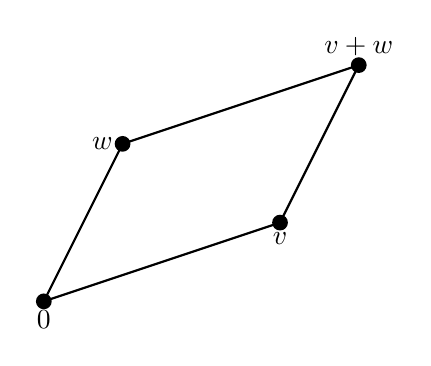
\begin{tikzpicture}[scale=1pt]
      \draw[thick] (0,0) -- (3,1) node[below] {};
      \draw[thick] (0,0) -- (1,2) node[left] {};
      \draw[thick] (1,2) -- (4,3) node[above] {};
      \draw[thick] (3,1) -- (4,3) node[right] {};
      \fill (3,1) circle (0.1) node[below] {$v$};
      \fill (1,2) circle (0.1) node[left] {$w$};
      \fill (0,0) circle (0.1) node[below] {$0$};
      \fill (4,3) circle (0.1) node[above] {$v+w$};
    \end{tikzpicture}
  \end{figure}
 
 
  By the above discussion, $f$ sends this parallelogram 
  to another parallelogram whose vertices are 
  $0$, $f(v)$, $f(w)$, and $f(v+w)$. By the geometric 
  interpretation of vector addition, this means that 
  $f(v+w) = f(v)+f(w)$. A similar argument works for 
  subtraction.

  Now, if $w\in \mathrm{Span}(v)\cap U$, then choose some 
  $u\in U\ssm \mathrm{Span}(v)$, and apply the above argument to 
  the pair $w-u$ and $v+u$, and then to the pairs 
  $w,u$ and $v,u$ to get $f(v+w) = f(v) + f(w)$.

  Let $v\in U\ssm \{0\}$ and $\alpha \in \R\ssm 0$ be such that 
  $\alpha v\in U$. We can write $f(\alpha v) = g(\alpha,v)f(v)$, and
  we need to show that $g$ does not depend on $v$. Let
  $w\in U\ssm \mathrm{Span}(v)$ be such that $\alpha w\in U$, 
  and consider the following line configuration:
  \begin{figure}[!h]
    \centering
    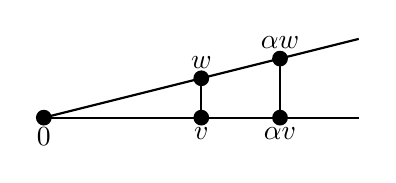
\begin{tikzpicture}
      \draw[thick] (0,0) -- (4,0) node[below] {};
      \draw[thick] (0,0) -- (4,1) node[left] {};
      \draw[thick] (2,0) -- (2,0.5) node[above] {};
      \draw[thick] (3,0) -- (3,0.75) node[above] {};
      \fill (0,0) circle (0.1) node[below] {$0$};
      \fill (2,0.5) circle (0.1) node[above] {$w$};
      \fill (2,0) circle (0.1) node[below] {$v$};
      \fill (3,0.75) circle (0.1) node[above] {$\alpha w$};
      \fill (3,0) circle (0.1) node[below] {$\alpha v$};
    \end{tikzpicture}
  \end{figure}


  Where the lines $(v,w)$ and $(\alpha v,\alpha w)$ are parallel. 
  Since $f$ preserves line configurations and paralellism, if 
  $f(\alpha v) = \beta f(v)$, then 
  $f(\alpha w) = \beta f(w)$. The case when 
  $w\in \mathrm{Span}(v)$ is treated similarly to additivity. 
  Overall, we get that $g$ as defined above 
  does not depend on $v$.

  Moreover, it is easy to check that wherever 
  $g$ is defined, $g(\alpha+\beta) = g(\alpha) + g(\beta)$ 
  and $g(\alpha\beta) = g(\alpha)g(\beta)$, and hence 
  is a restriction of a field 
  automorphism of $\R$, and hence is the identity.
\end{proof}
Note that we have actually proved a stronger result 
for a general field:
\begin{theorem}
  Let $\K$ be a field with at least three elements, and 
  let let $n>1$. Let $f:\K^n\to \K^n$ be a bijection sending 
  affine subspaces to affine subspaces. Then 
  there exists $z\in \K^n$ such that for all 
  $x,y\in \K^n$ and $\alpha\in \K$,
  \begin{align*}
    f(\alpha x + y) = g(\alpha)f(x) + f(y) + z
  \end{align*}
  Where $g:\K\to\K$ is a field automorphism.

  Such a function is called \textit{semilinear}
\end{theorem}
We can prove this by taking $U = \K^n$ and following the same argument. 
The condition $|\K|\ge 3$ is to be able to characterize 
parallel lines as disjoint lines lying in the same affine plane.

Using this, we can complete the construction of the main tool of this
section -- that any map projection which preserves convex sets can be
written as the composition of the gnomonic projection and an affine
linear transformation of the plane.

\begin{theorem}
  Let $\psi:U\to \R^2$ be a map projection 
  defined on a subset of the lower-hemisphere, and let 
  $\vphi$ be the gnomonic projection. If $\psi^{-1}$ sends 
  convex sets to convex sets, then there exists an affine linear map 
  $L$ such that $\psi = L\circ \vphi$.
\end{theorem}
\zs{this field automorphism business feels a little too abstract for the audience. In order to show $f$ is linear, you need to show $f(u+v) = f(u)+f(v)$ and $f(kx) = kf(x)$ and preserving parallelograms is strong enough to imply both of these. You showed additivity, and scaling is even easier. If a parallelogram is preserved, it sends parallel segments of equal length to parallel segments of equal length, and this extends to the statement that any pair of parallel segments has the ratio of their lengths preserved, so any pair of collinear segments have the ratio of their length preserved, which implies linear.}
\begin{proof}
  By Lemma ~\ref{lem:gnomonic_convex}, the map $\vphi\circ
  \psi^{-1}:\psi(U)\to \R^2$ sends convex sets to convex sets. It is
  bijective on its range, since $\psi$ and $\vphi$ are bijective, and
  hence satisfies the conditions of Theorem
  ~\ref{thm:geometric_algebra}, meaning that there exists an affine
  linear isomorphism $L^{-1}:\R^2\to \R^2$ such that $\vphi = \psi
  \circ L^{-1}$.  Thus, $\psi = \vphi \circ L$, as desired.
  \mute{
  By the previous lemma, the gnomonic projection does indeed preserve
  convex sets.   If a map projection preserves convex sets, it must in
  particular preserve the one-dimensional convex sets, meaning it maps
  segments of great circles on the sphere to line segments in the
  plane.  Take $\psi$ and $\varphi$ to convexity-preserving map
  projections, and, without loss of generality take $\varphi$ to be
  the standard gnomonic projection described above. We consider the
  composition $\psi\varphi^{-1}$, which is a transformation of the
  plane which preserves convex sets, so in particular it sends line
  segments to line segments.  Since these transformations also
  preserve containment, we can additionally observe that
  $\psi\varphi^{-1}$ preserves \textit{collinearity} in the plane,
  which means it is an affine linear transformation of the plane.
  Since we can write $\psi$ as $\psi\varphi^{-1}\varphi$, we have
  successfully written our convexity-preserving map as the composition
  of the gnomonic projection and an affine linear transformation of
  the plane.}
\end{proof}
\zs{we don't use this anywhere. it's cute, but I don't think it's relevant}



\subsection{Stereographic Projection}

\zs{defn 9, lem 5 lem 6 lem 7 lem 8}

\begin{definition}
  The \textbf{stereograpic projection} from the sphere to the plane is
  defined by placing the plane tangent to the sphere at the south
  pole, and for any point $p$ on the sphere other than the north pole,
  $p$ is sent to the unique point $q$ in the plane which is on the
  line in 3-space passing through the north pole and $p$.

  If $(x,y,z)$ is a point on the sphere, then the action of the
  stereographic projection is
  \begin{align*}
    (x,y,z)\mapsto \left(\frac{x}{1-z},\frac{y}{1-z}\right)
  \end{align*}
  and its inverse, for $(u,v)$ in the plane:
  \begin{align*}
    (u,v)\mapsto \left( \frac{2u}{1+u^2+v^2},\frac{2v}{1+u^2+v^2},
    \frac{u^2+v^2-1}{1+u^2+v^2}   \right)
  \end{align*}
\end{definition}

What is somewhat surprising is that this projection sends every cap on
the sphere which doesn't pass through the north pole to a circle in
the plane.  There are several proofs of this fact, and we present
a rather straightforward algebraic one here.

\abn{This is a fact that is usually taught at a second 
year complex analysis course - perhaps we can leave this out if 
we want to conserve space?}
\begin{lemma}
  The stereographic projection sends every cap which does not pass through the north pole to a circle in the plane.
\end{lemma}
\begin{proof}
  We proceed algebraically.  Since a cap on the sphere can be
  identified by the plane in $\R^3$ which intersects the sphere along
  its boundary, we can parametrize such a cap by writing the equation
  for its corresponding plane, $ax+by+cz=d$, restricting $(x,y,z)$ to
  be points on the sphere.  The image in the plane of this cap is some
  set of $(u,v)$ points, and we can explicitly write this by
  substituting in for $x$, $y$, and $z$ the corresponding values for
  the inverse stereographic projection.  We write
  $\mathcal{W}=u^2+v^2$ for the ease of presentation. 

  \begin{align*}
    d&=ax+by+cz\\
    d&=a\left(\frac{2u}{1+u^2+v^2}\right)+b\left(\frac{2v}{1+u^2+v^2}\right)+c\left(\frac{u^2+v^2-1}{1+u^2+v^2}\right),
    \text{ by substitution}\\
    d&=a\left(\frac{2u}{1+\mathcal{W}}\right)+b\left(\frac{2v}{1+\mathcal{W}}\right)+c\left(\frac{\mathcal{W}-1}{1+\mathcal{W}}\right),
    \text{ by change-of-variable }\mathcal{W}=u^2+v^2\\
    d\left(1+\mathcal{W}\right)&=2au+2bv+c\left(\mathcal{W}-1\right),
    \text{ multiplying through by }1+\mathcal{W}\\ 0 &=
    (c-d)\mathcal{W} + 2au +2bv - c - d,\text{ by rearrangement}\\
    0 &= (c-d)(u^2+v^2)+2au+2bv - c - d,\text{ by change-of-variable
    } \mathcal{W}=u^2+v^2 
  \end{align*}

  This last line is the equation of a circle in the plane if $c\neq d$
  and a line otherwise.  Since $c=d$ if and only if the point
  $(x,y,z)=(0,0,1)$ (i.e. the north pole) is on the plane, and we
  assumed that this is not the case, we have shown that the image
  under the stereographic projection of every cap which does not pass
  through the north pole is a circle in the plane.

\end{proof}

We now have in-hand a circle-preserving map projection, and we now
turn to demonstrating that the stereographic projection is essentially
the unique map projection with this property.  We can observe that if
we perform stereographic projection and compose it with
a transformation of the plane which sends every circle to a circle,
then this composition is a circle-preserving map projection.  The next
lemma demonstrates that the class of transformations of the plane
which preserve circles is actually quite narrow.

\begin{lemma}
  If $T$ is a transformation of the plane which sends every circle in
the plane to another circle, then $T$ must be a linear transformation
which is the composition of a scaling, a rotation, a reflection, and
a translation, i.e. a scaled isometry.  
\end{lemma}
\begin{proof}

  We first argue that if we restrict our attention to \textit{linear}
  transformations, the scaled isometries are the only transformations
  which preserve circles.  

  If $T$ is a scaled isometry with scaling factor $\alpha$, then, by
  definition, for any points $x$ and $y$, the distance between $T(x)$
  and $T(y)$ is $\alpha$ times the distance between $x$ and $y$.
  Therefore, if we choose a circle $Y$ of radius $r$ and let $x$ be
  the center, then for any $y\in Y$, $d(T(x),T(y)) = \alpha r$, so
  $T(Y)$ is a circle of radius $r$.

  Next, if $T$ is a linear transformation which is \textit{not}
  a scaled isometry, then we can find three points $x$, $y$, and $z$
  such that $d(T(x),T(y)) = \alpha d(x,y)$ but $d(T(x),T(z)) \neq
  \alpha d(x,z)$.  Furthermore, since linear transformations preserve
  ratios of lengths of collinear segments, and we have two segments
  whose ratios of lengths are not preserved, these three points cannot
  be collinear, so we can consider the circle centered at $x$ and
  passing through $y$ and $z$.  But, since the ratio of lengths isn't
  preserved, $T$ distorts this circle, so $T$ is not
  circle-preserving.

  We next need to rule out the existence of a non-linear
  transformation $T$ which is circle preserving.  We proceed by
  contradiction.  Suppose that $T$ is non-linear and
  circle-preserving.  Then, since $T$ is non-linear, there is some
  line $\ell$ such that the image $T(\ell)$ is not a line, so we can
  find three points $x$, $y$, and $z$ which are collinear, but $T(x)$,
  $T(y)$, and $T(z)$ are not.  Therefore, we can find a unique circle
  $C_T$ passing through $T(x)$, $T(y)$, and $T(z)$.  Let $T(a)$ be
  some other point on this circle, and we consider the preimage of
  this point, $a$.  If $a$ is not on the line $\ell$, then we can
  construct two circles, one passing through $a$, $x$, and $y$ and one
  passing through $a$, $y$, and $z$.  These two circles intersect at
  only two points, $a$ and $y$, but both of these circles are sent to
  $C_T$ by $T$, which is impossible if $T$ is injective.  Therefore,
  $a$ must lie on the line $\ell$.

  By repeating this argument, any point on the circle $C_T$ must be
  the image of some point on $\ell$.  By continuity, we can see that
  every point on $\ell$ is sent to a point on $C_T$, but the
  homeomorphic image of a line cannot be a circle, so such
  a non-linear $T$ cannot exist.

  Thus, a transformation of the plane is circle-preserving if and only
  if it is a scaled isometry.
\end{proof}

We can put these two pieces together to prove the main tool of this
section -- that any map projection from the sphere to the plane which
preserves circles is the composition of the stereographic projection
and a scaled isometry.

\begin{lemma}
  The map projections from the sphere to the plane which send every
  cap to a circle are exactly those which can be written as the
  composition of the stereographic projection followed by a scaled
  isometry of the plane.
\end{lemma}
\begin{proof}
  Let $\varphi$ and $\psi$ be two map projections which preserve
  circles, and without loss of generality let $\varphi$ be the
  standard stereographic projection.  Then the composition
  $T=\psi\circ\varphi^{-1}$ is a transformation of the plane which
  preserves circles, so by the previous lemma, $T$ is a scaled
  isometry.  Then, we can write $\psi= T^{-1}\varphi$, which is the
  composition of the stereographic projection and a scaled isometry.
\end{proof}

As in the previous section, we can construct an example of two regions
whose Reock scores are permuted by the stereographic projection.  In
fact, we can use \textit{exactly} the same pair of regions as in the
convex hull settings, as is made clear by the following lemma.

\begin{lemma}
  Let $\varphi$ be the stereographic projection and $C_\theta$ be
  a spherical cap centered at the south pole parametrized by the angle
  $\theta <\pi/4$ formed between the central axis of the sphere and
  the line of projection passing through the north pole and the
  boundary of the cap (Figure~\ref{fig:stereocap}). Then
  $\phi(C_\theta)$ is a disk in the plane, centered at the origin, and
  has radius $2\tan\theta$
\end{lemma}
\begin{figure}
  \centering
  \includegraphics[width=.8\textwidth]{figs/stereo_cap.jpg}\\
  \caption{ The image of a cap with angle $\theta$ between the polar axis and the line of projection is a circle of radius $2\tan\theta$.  }
  \label{fig:stereocap}
\end{figure}
\begin{proof}


  Since $\varphi$ projects from the north pole of the sphere and the
  sphere's south pole is mapped to the origin in the plane, the image
  of $C_\theta$ is totally radially symmetric about the origin, and is
  therefore a circle.  To see that its radius is $2\tan(\theta)$,
  place the south pole of the sphere tangent to the plane at the
  origin. By construction, for any point $p$ on the boundary of
  $C_\theta$, there is a unique line passing through the north pole of
  the sphere, $p$, and the point $\varphi(p)$ on the boundary of the
  disk in the plane.  By definition, this line meets the central axis
  of the sphere at an angle of $\theta$, and the central axis of the
  sphere meets the plane orthogonally, so the center of the sphere,
  the origin, and the point $\varphi(p)$ form a right triangle with
  angle $\theta$.  Since we know that the distance between the north
  pole of the sphere and the origin is 2, we can write the distance
  between the origin and $\varphi(p)$ as $2\tan(\theta)$.

\end{proof}

\begin{theorem}
	Let $A$ be a region on the sphere.  Then there exist two regions $\kappa'_N,\kappa'_S\subset A$ such that the Reock scores of $\kappa'_N$ and $\kappa'_S$ are equal on the sphere, but under the stereographic projection $\varphi$, the Reock score of $\kappa'_S$ is strictly greater than that of $\kappa'_N$. 
\end{theorem}

\begin{proof}
	First, since $A$ is a region, we can find some cap $\kappa$ inside of $A$ such that the center of $\kappa$ is not the south pole of the sphere, and the north pole is exterior to $\kappa$.  This cap is bisected by a line of longitude, in particular the great circle which passes through the two poles and the center of $\kappa$.  This line of longitude meets $\kappa$ at exactly two points, and we call $p_N$ the point closer to the north pole and $p_S$ the point closer to the south pole.
	
	Choose some $r$ strictly less the radius of $\kappa$ and let $\kappa'_S$ be the region constructed by deleting a cap of radius $r$ from the interior of $\kappa$ tangent at $p_S$.  Construct $\kappa'_N$ analogously by deleting a cap of radius $r$ tangent at $p_n$. Observe that the Reock scores of $\kappa'_N$ and $\kappa'_S$ are identical, since each has the boundary of $\kappa$ as its smallest bounding cap and both figures have the same area.
	
	We now consider the images of $\kappa'_N$ and $\kappa'_S$ under the stereographic projection $\varphi$.  Since $\varphi$ preserves points of tangency, containment, and sends every cap away from the north pole to a circle, the images $\varphi(\kappa'_N)$ and $\varphi(\kappa'_S)$ are both regions which are disks with a smaller disk, tangent to a point on the circumference, deleted.  Furthermore, since the boundary of $\kappa$ was the smallest bounding cap of both regions on the sphere, the image of the boundary of $\kappa$ under $\varphi$ is the smallest bounding circle of the images of these regions in the plane.
	
	We can now observe that these two regions in the plane do not have the same Reock score.  Both have the same bounding circle, but $\varphi(\kappa'_N)$ is strictly smaller than $\varphi(\kappa'_S)$.  This is because the stereographic projection distorts areas in a way such that figures further from the south pole have their areas magnified more than the same region closer to the south pole.  If the regions in question are sufficiently small, letting $\theta$ denote the polar angle at which we consider a small cap on the sphere, a cap of radius $r$ will be sent to a circle with radius roughly $r/\cos^2{\theta}$\zs{check  this}, and a straightforward examination of this as a function of $\theta$ shows that it grows faster as $\theta$ increases.
	
	Since $\varphi(\kappa'_N)$ fills a smaller fraction of the bounding circle than $\varphi(\kappa'_N)$ does, its Reock score is strictly worse, and the stereographic projection does not preserve Reock scores.
\end{proof}


\section{Convex Hull}\label{sec:ch}
We next consider the \textit{convex hull
score}.  We briefly recall the definition of a convex set and then
define this score function.


\begin{definition}
	A set in a metric space is \textbf{convex} if the shortest geodesic segment between any two points in the set is entirely 
	contained within that set.
\end{definition}



\begin{figure}[h]
	\centering
	%\includegraphics[width=.35\textwidth]{figs/ch_example.png}
	
\definecolor{qqqqff}{rgb}{0,0,1}
\begin{tikzpicture}[scale=2,line cap=round,line join=round,>=triangle 45,x=1cm,y=1cm]
\clip(-3.1808855374298814,0.7054196919809391) rectangle (2.8436799719688346,4.78259146738453);
\draw [line width=2pt,color=qqqqff] (-0.5403387932320529,4.199917026631047)-- (-1.4876311065851997,3.283901898015972);
\draw [line width=2pt,color=qqqqff] (-2.59555742277687,2.1884264530340003)-- (-1.030093019846988,1.0427513872026393);
\draw [line width=2pt,color=qqqqff] (-1.030093019846988,1.0427513872026393)-- (-0.4266458477678716,2.503268455857886);
\draw [line width=2pt,color=qqqqff] (-0.4266458477678716,2.503268455857886)-- (1.1213273327829054,2.310865009687734);
\draw [line width=2pt,color=qqqqff] (1.1213273327829054,2.310865009687734)-- (0.6315731061679702,3.8850750238071616);
\draw [shift={(-2.4623421270336228,3.1638741521373337)},line width=2pt,color=qqqqff]  plot[domain=-1.7065250247888804:0.12252504290266225,variable=\t]({1*0.9845021730326186*cos(\t r)+0*0.9845021730326186*sin(\t r)},{0*0.9845021730326186*cos(\t r)+1*0.9845021730326186*sin(\t r)});
\draw [shift={(-0.01568921678809781,3.814254744830714)},line width=2pt,color=qqqqff]  plot[domain=0.10898159374480773:2.5077053734556625,variable=\t]({1*0.6511252004282949*cos(\t r)+0*0.6511252004282949*sin(\t r)},{0*0.6511252004282949*cos(\t r)+1*0.6511252004282949*sin(\t r)});
\draw [line width=2.8pt] (-2.685655712545722,2.2031756923666004)-- (-1.0153159792750968,0.9768503185729869);
\draw [line width=2.8pt] (-1.0153159792750968,0.9768503185729869)-- (1.158637184087576,2.29171136125267);
\draw [line width=2.8pt] (1.158637184087576,2.29171136125267)-- (0.6620716009713541,4.04266375305702);
\draw [shift={(-0.01540854579167931,3.8076224532316205)},line width=2.8pt]  plot[domain=0.33394133978769747:2.3774678762164125,variable=\t]({1*0.7170939700497241*cos(\t r)+0*0.7170939700497241*sin(\t r)},{0*0.7170939700497241*cos(\t r)+1*0.7170939700497241*sin(\t r)});
\draw [line width=2.8pt] (-2.685655712545722,2.2031756923666004)-- (-0.5331419341269765,4.30378361705294);
\draw [color=qqqqff](-0.7863560820341027,3.2000351515748306) node[anchor=north west] {\LARGE$\Omega$};
\draw (0.1549822788094467,1.5938421717062845) node[anchor=north west] {\LARGE$\mathrm{CH}(\Omega{)}$};
\end{tikzpicture}

	\caption{A region $\Omega$ and its convex hull.}
	\label{fig:ch_example}
\end{figure}

\begin{definition}
  Let $\mathrm{conv}(\Omega)$ denote the \textit{convex hull} of
  a region $\Omega$ in either the sphere or the plane, which is the
  smallest convex region containing $\Omega$.  Then we define the
  \textit{convex hull score} of $\Omega$ as 
  \begin{align*}
    \mathrm{CH}(\Omega)=
    \frac{\mathrm{area}(\Omega)}{\mathrm{area}(\mathrm{conv}(\Omega))}
  \end{align*}
\end{definition}



Throughout this section, let $\vphi:\Omega \to \R^2$ be a 
map projection defined on a patch of the sphere $\Omega\subset \mbb{S}^2$.


We begin by observing that such a projection must preserve certain geometric properties within these patches.
\begin{lemma}~\label{lem:CH_prep}
	If $\vphi$ preserves the ordering of regions induced by their convex hull scores, then the following must 
	hold:
	\begin{enumerate}
		\item $\vphi$ and $\vphi^{-1}$ send convex regions to convex regions
		\item $\vphi$ sends every segment of a great circle on the sphere to a line segment in the plane.  That is, it preserves geodesics.
		\item There exists a region $U$ in our patch
		such that for any regions $A,B\subset U$, if 
		$A$ and $B$ have equal area on the sphere, then 
		$\vphi(A)$ and $\vphi(B)$ have equal area in the plane.  The same holds 
		for $\vphi^{-1}$ for all pairs of regions inside of $\vphi(U)$.
	\end{enumerate}
\end{lemma}

\begin{figure}[h]
	\centering
	%\includegraphics[width=.25\textwidth]{figs/ch_sphere_schema.png}
	\definecolor{ffffff}{rgb}{1,1,1}


\begin{tikzpicture}[scale=.35,line cap=round,line join=round,>=triangle 45,x=1cm,y=1cm]

\clip(-6.762534270657285,-7.4038512549636435) rectangle (12.125044594505917,5.378465301245481);
\draw [line width=3.6pt,fill=black,fill opacity=0.27] (2.52,-1.24) circle (5.094349811310566cm);
\draw [line width=0.4pt,color=ffffff,fill=ffffff,fill opacity=1] (2.82,-2.62) circle (1.352035502492446cm);
\draw [rotate around={-134.1620339448981:(0.25635345523487,0.2782885419108182)},line width=0.4pt,color=ffffff,fill=ffffff,fill opacity=1] (0.25635345523487,0.2782885419108182) ellipse (1.6381871321999442cm and 0.5964014274522406cm);
\draw [rotate around={2.00955381302114:(1.84,1.24)},line width=0.4pt,color=ffffff,fill=ffffff,fill opacity=1] (1.84,1.24) ellipse (1.2329931677283157cm and 0.46805144125908144cm);
\draw (-0.14942211242749375,1.2652523257265278) node[anchor=north west] {\LARGE$A$};
\draw (2.089030655746763,-1.9839442053140297) node[anchor=north west] {\LARGE$B$};
\draw (5.613994458370557,4.161101819701755) node[anchor=north west] {\LARGE$U$};
\end{tikzpicture}
	\caption{Two equal area regions $A$ and $B$ removed from $U$.}
	\label{fig:ch_schema}
\end{figure}



\begin{proof}
	\ \\
	
	\vspace*{-2em}
	\begin{enumerate}
		\item[] The proof of (1) follows from the idea that any projection which preserves the convex hull score ordering of regions must 
		preserve the maximizers in that ordering.   Here, the maximizers are convex sets.
		
		\item[]  Suppose, for the sake of contradiction, that there is some geodesic segment $s$ on the sphere such that $\vphi(s)$ is not a line segment. Take $s$ and 
		consider its $\eps$-thickening, which is the region defined by the union of $\eps$ caps centered at each point 
		along the segment.  We can observe that since $\vphi(s)$ is not a line segment, there is some small $\delta$ such that the $\delta$-thickening of $\vphi(s)$ is not convex.  
		
		The $\eps$-thickening of $s$ is convex for all $\eps$, so by (1), $\vphi$ will send this to a convex region.  However, there must be some $\eps'$ such that the $\eps'$-thickening of $s$ is sent to the $\delta$-thickening of $\vphi(s)$, which contradicts the fact that the image of these thickenings are convex.
		
		The proof that $\vphi^{-1}$ sends line segments in the plane to great circle segments on the sphere is analogous.  
		
		This proves (2).
		
		
		
\item[] To show (3), let our region $U\subset\Omega$ be a cap, without loss of generality.  Take $A,B$ to be regions of equal area such that $A$ and $B$ are properly contained in the interior of $U$, as in \Cref{fig:ch_schema}.  Define two new regions $X=U\ssm A$ and $Y=U\ssm B$, i.e. these regions are equal to $U$ with $A$ or $B$ deleted, respectively.  

The cap $U$ is itself the convex hull of both $X$ and $Y$, and since $A$ and $B$ have equal area, we have that $\mathrm{CH}(X) = \mathrm{CH}(Y)$.  Since $U$ is a cap, it is convex, so by (1), $\vphi(U)$ is also convex.  Since $\vphi$ preserves the ordering of convex hull scores and $X$ and $Y$ had equal scores on the sphere, $\vphi$ must send $X$ and $Y$ to regions in the plane which also have the same convex hull score.  Furthermore, the convex hulls of $\vphi(X)$ and $\vphi(Y)$ are $\vphi(U)$.

We can then write 
\begin{align*}
\mathrm{CH}(X) &= \mathrm{CH}(Y)\\
\ &\\
\frac{\mathrm{Area}(\vphi(X))}{\mathrm{Area}(\vphi(U))} &= \frac{\mathrm{Area}(\vphi(Y))}{\mathrm{Area}(\vphi(U))}\\
\ &\\
\frac{\mathrm{Area}(\vphi(U)) - \mathrm{Area}(\vphi(A))}{\mathrm{Area}(\vphi(U))} &= \frac{\mathrm{Area}(\vphi(U)) - \mathrm{Area}(\vphi(B))}{\mathrm{Area}(\vphi(U))}\\
\ &\\
\mathrm{Area}(\vphi(A)) &= \mathrm{Area}(\vphi(B))
\end{align*}
 which is what we wanted to show.  The proof that $\vphi^{-1}$ also has this property is analogous.  This proves (3).
\end{enumerate}
\end{proof}

We can now show that no map projection can preserve the convex hull score ordering of regions by proving that there is no projection from a patch on the sphere to the plane which has all three of the properties described above in \Cref{lem:CH_prep}. 


\begin{theorem}
	There does not exist a map projection satisfying the 
	conditions in Lemma~\ref{lem:CH_prep}
\end{theorem}
\begin{proof}
	Assume that such a map, $\vphi$, exists, and restrict 
	it to $U$ as above. Let $T\subset U$ be a 
	spherical equilateral triangle with 
	$\mathrm{Diam}(T)<\frac{\mathrm{Diam}(U)}{3}$, centered at 
	the center of $U$. Let $T_1$ and $T_2$ be two 
	congruent triangles meeting at a point and 
	each sharing a face with $T$, as in \Cref{fig:sphtris}.

\begin{figure}[h]
	\centering
	\includegraphics[width=.25\textwidth]{figs/spheretri.png}
	\caption{The spherical regions $T,T_1,T_2$.}
	\label{fig:sphtris}
\end{figure}












We first argue that the images of $T\cup T_1$ and $T\cup T_2$ are parallelograms.

Without loss of generality, consider. $T\cup T_1$.  By construction, it is a 
convex spherical quadrilateral. By symmetry, its geodesic 
diagonals on the sphere divide it into four triangles of equal area, since the long diagonal splits $T$ and $T_1$ in 
half, and $T$ and $T_1$ have the same area.


		Since $\vphi$ sends spherical geodesics to line segments in the plane, it must send 
		$T\cup T_1$ to a Euclidean quadrilateral $Q$ whose diagonals 
		are the images of the diagonals of the spherical quadrilateral $T\cup T_1$.
		
		 Since 
		$\vphi$ sends equal area regions to equal area 
		regions, it follows that the diagonals 
		of $Q$ split it into four equal area triangles.
		
		We now argue that this implies that $Q$ is a Euclidean parallelogram by showing that its diagonals bisect each other.  Since the four triangles 
		formed by the diagonals of $Q$ are all the same area, we can pick two of these triangles which share a side 
		and consider the larger triangle formed by their union.  One side of this triangle is a diagonal $d_1$ of $Q$ and its area is 
		bisected by the other diagonal $d_2$, which passes through $d_1$ and its opposite angle.  This area bisector passes through the midpoint of the side $d_1$, meaning that the diagonal $d_2$ bisects the diagonal $d_1$.  Since this holds for any choice of two adjacent triangles in $Q$, the diagonals must bisect each other, so $Q$ is a parallelogram.
		
		
\begin{figure}[h]
	\centering
	\includegraphics[width=.25\textwidth]{figs/spheretri_plane.png}
	\caption{The image under $\vphi$ of $T,T_1,T_2$.}
	\label{fig:sphtris_pl}
\end{figure}

Since $T\cup T_1$ and $T\cup T_2$ are both spherical quadrilaterals which overlap on the spherical triangle $T$, the images of $T\cup T_1$ and $T\cup T_2$ are Euclidean parallelograms of equal area which overlap on a shared triangle $\vphi(T)$.
	Therefore, the image of $T\cup T_1\cup T_2$ must 
	consist of two parallelograms, one of whose 
	edges is the diagonal of the other. In other words, 
	$\vphi(T\cup T_1\cup T_2)$ is a Euclidean trapezoid 
	whose boundary consists of four Euclidean geodesic 
	segments, as in \Cref{fig:sphtris_pl}.
	
	To find the contradiction, consider the point on the sphere at which $T$, $T_1$, and $T_2$ meet.  Since these triangles are all equilateral spherical triangles, the three angles at this point are each at least $\tfrac{\pi}{3}$ radians, because the sum of interior angles on a triangle is at least $\pi$.  Therefore, the total measure of the three angles at this point is at least $\pi$.  Therefore, the two geodesic segments which are part of the boundaries of $T_1$ and $T_2$ meet at this point at an angle of measure at least $\pi$, so together they do not form a geodesic.  Therefore, on the sphere, the region $T\cup T_1\cup T_2$ has a boundary consisting of five geodesic segments whereas its image has a boundary consisting of four, which contradicts the assumption that $\vphi$ and $\vphi^{-1}$ preserve geodesics.
\end{proof}

This implies that no map projection can preserve the ordering of regions by their convex hull scores, which is what we aimed to show.

\section{Reock}\label{sec:reock}

Let $\mathrm{circ}(\Omega)$ denote the \textit{smallest bounding
circle} (smallest bounding \textit{cap} on the sphere) of a region
$\Omega$.  Then the \textit{Reock score} of $\Omega$ is 

$$\mathrm{Reock}(\Omega)=
\frac{\mathrm{area}(\Omega)}{\mathrm{area}(\mathrm{circ}(\Omega))}.$$

In words, it is the ratio of the area of the region to the area of the
smallest circle containing that region, and it is equal to one if and
only if $\Omega$ is a circle.  

Since $\mathrm{Reock}(\Omega)=1$ if and only if $\Omega$ is a circle,
we can observe that any candidate $\vphi$ for a map projection 
which preserves the ordering of Reock scores must, at the 
very least, preserve the maximizeres in the ordering, meaning 
it sends caps on the sphere to circles in the plane.  

By Theorem~\ref{thm:stereographic_mobius}, we know that any projection which sends every cap on the sphere to a 
circle in the plane is the composition of the stereographic projection with a M\"obius transformation of the plane and possibly a reflection.  Equivalently, we can realize any such projection as a M\"obius transformation of the \textit{sphere} followed by the stereographic projection.  On the sphere, all of the transformations which generate the  M\"obius transformations preserve Reock scores and therefore the ordering of regions induced by these scores. 

If we can show that the stereographic projection does not preserve Reock scores, then it cannot be the case that any map projection does so, because the stereographic projection will distort the ordering, no M\"obius transformation can correct this distortion, and no other transformation can either, since this would cause some cap to be sent to a non-circle.


\begin{theorem}\label{thm:reock}
  Let $A$ be a region on the sphere.  Then there exist two regions
  $\kappa'_N,\kappa'_S\subset A$ such that the Reock scores of
  $\kappa'_N$ and $\kappa'_S$ are equal on the sphere, but under the
  stereographic projection $\varphi$, the Reock score of $\varphi(\kappa'_S)$
  is strictly greater than that of $\varphi(\kappa'_N)$. 
\end{theorem}


\begin{proof}


  We prove this constructively.  Fix a half-great circle passing through the north and south poles of the sphere (i.e. a \textit{line of longitude} on the Earth).  Each of the figures described will be constructed from spherical caps with their centers on this half-great circle.  Furthermore, observe that we can specify any point on this half-great circle by giving its polar angle $\theta$, which is the angle formed by the lines (in $\R^3$) which are the polar axis of the sphere and the line passing through the north pole of the sphere and our point of interest.  Recall that this second line is the one used to determine the point $q$ in the plane to which a point $p$ on the sphere is sent.
  
  
  We prove this in the case of the unit sphere, and the general result for the sphere of radius $\mc{R}$ follows from applying a scaling factor at the end.
  
  Choose two angles $\theta_S$ and $\theta_N$ such that $0\leq\theta_S<\theta_N<\tfrac{\pi}{2}$.  These two angles identify a cap $\kappa$ centered on our half-great circle where $\theta_S$ is the polar angle which gives the point on the cap closest to the south pole and $\theta_N$ the north pole.  Choose another angle $\theta_D <\tfrac{\theta_N-\theta_S}{2}$.  We can similarly construct two more caps $\kappa_N$ using the angles $\theta_N$ and $\theta_N - \theta_D$ and $\kappa_S$ using the angles $\theta_S$ and $\theta_S+\theta_D$.  Each of these two caps is fully contained in $\kappa$ and are tangent to it at the shared boundary point.  A cross-section along our line of longitude is shown in \Cref{fig:reock_sphere_schema}.
  
  
  \begin{figure}[h]
  	\centering
  	%\includegraphics[width=.5\textwidth]{figs/reock_sph_schema.png}
  	\definecolor{ffwwqq}{rgb}{1,0.4,0}
\definecolor{qqttcc}{rgb}{0,0.2,0.8}
\begin{tikzpicture}[line cap=round,line join=round,>=triangle 45,x=1cm,y=1cm]
\clip(-3.059616031054939,-5.482081270032577) rectangle (9.99814205103663,6.011797314398574);
\draw [shift={(1.39,0.41)},line width=2.5pt]  plot[domain=-1.6009682543555996:1.540624399234193,variable=\t]({1*4.972263066250617*cos(\t r)+0*4.972263066250617*sin(\t r)},{0*4.972263066250617*cos(\t r)+1*4.972263066250617*sin(\t r)});
\draw [line width=2.5pt] (1.54,5.38)-- (5.827220035894456,2.6537643265407334);
\draw [line width=2.5pt,dashed,color=qqttcc] (1.54,5.38)-- (6.248241510524688,1.468720655043056);
\draw [line width=2.5pt,dashed,color=ffwwqq] (1.54,5.38)-- (4.287651725431555,-3.63067005311044);
\draw [line width=2.5pt] (1.54,5.38)-- (3.2041318882884013,-4.219505966287888);
\draw [shift={(-3.44,-0.94)},line width=2.5pt,color=qqttcc]  plot[domain=0.23697883378697754:0.3678716704111534,variable=\t]({1*10.308093907216794*cos(\t r)+0*10.308093907216794*sin(\t r)},{0*10.308093907216794*cos(\t r)+1*10.308093907216794*sin(\t r)});
\draw [shift={(-1.36,5)},line width=2.5pt,color=ffwwqq]  plot[domain=5.174361549076037:5.291583521566141,variable=\t]({1*10.679475642558485*cos(\t r)+0*10.679475642558485*sin(\t r)},{0*10.679475642558485*cos(\t r)+1*10.679475642558485*sin(\t r)});
\draw [shift={(1.14,0.48)},line width=2.5pt]  plot[domain=-1.146403466819911:0.41822432957922906,variable=\t]({1*5.925672957563554*cos(\t r)+0*5.925672957563554*sin(\t r)},{0*5.925672957563554*cos(\t r)+1*5.925672957563554*sin(\t r)});
\draw (5.691369061245417,3.5324761595710585) node[anchor=north west] {\color{qqttcc}\LARGE$\kappa_N$};
\draw (2.465325805609785,-4.401351535876993) node[anchor=north west] {\color{ffwwqq}\LARGE$\kappa_S$};
\draw (6.886529002546884,-0.7488678952988525) node[anchor=north west] {\LARGE$\kappa$};
\end{tikzpicture}
  	\caption{The points along the line of longitude which define the three caps of interest.  $\kappa_N$ and $\kappa_S$ are the same size and defined by angles of the same measure.}
  	\label{fig:reock_sphere_schema}
  \end{figure}
  
  We define the region $\kappa_N'$ as $\kappa\ssm\kappa_N$ and $\kappa_S'$ as $\kappa\ssm\kappa_S$.  That is, each of these is formed by deleting the corresponding smaller cap from $\kappa$.  Since $\kappa_N$ and $\kappa_S$ have the same area and the smallest bounding cap of 
  $\kappa_N'$ and $\kappa_S'$ is just $\kappa$ itself, these two regions have identical Reock scores on the sphere.  
  Indeed, one can observe that $\kappa_N'$ is the 
  $180$ degree rotation of $\kappa_S'$ about the center of $\kappa$.
  
  However, under the stereographic projection, these regions no longer have the same Reock score in the plane.  The stereographic projection will send our half-great circle to a ray in the plane emanating from the origin and all spherical caps to planar circles, so the stereographic projection will send our spherical regions $\kappa_N'$ and $\kappa_S'$ to planar regions $\varphi(\kappa_N')$ and $\varphi(\kappa_S')$ which can be constructed from circles with their centers along this ray.
  
  The stereographic projection sends the point on the sphere on our half-great circle corresponding to angle $\theta$ to the point in the plane at distance $2\tan(\theta)$ from the origin along our ray.  Thus, $\varphi(\kappa)$ is a circle with diameter $2\tan(\theta_N)-2\tan(\theta_S)$, $\varphi(\kappa_S)$ has diameter $2\tan(\theta_S+\theta_D)-2\tan(\theta_S)$ and $\varphi(\kappa_N)$ has diameter $2\tan(\theta_N)-2\tan(\theta_N-\theta_D)$.  Similarly to their construction on the sphere, $\varphi(\kappa_N')$ and $\varphi(\kappa_S')$ are equal to $\varphi(\kappa)\ssm \varphi(\kappa_N)$ and $\varphi(\kappa)\ssm \varphi(\kappa_S)$, respectively.  We can further observe that $\varphi(\kappa)$ is the smallest bounding circle of both regions in the plane.
  
  However, these two regions do not have identical Reock score in the plane, since $\varphi(\kappa_S')$ has a larger area (and therefore strictly better Reock score) than $\varphi(\kappa_N')$.  To see this, we will show that the area of $\varphi(\kappa_N)$ is strictly \textit{greater} than that of $\varphi(\kappa_S)$. Since all of these regions are circles, it suffices to show that the diameter of $\varphi(\kappa_N)$ is strictly {greater} than that of $\varphi(\kappa_S)$.  We can write
  
  \begin{align*}
  \mathrm{diam}_{\varphi(\kappa_N)} - \mathrm{diam}_{\varphi(\kappa_S)} &= \left(2\tan(\theta_N) - 2\tan(\theta_N-\theta_D)\right) - \left( 2\tan(\theta_S+\theta_D) - 2\tan(\theta_S) \right)\\
  &= \left(\tan(\theta_N) - \tan(\theta_N-\theta_D)\right) - \left( \tan(\theta_S+\theta_D) - \tan(\theta_S) \right),
  \end{align*}
  
and the claim follows by showing that this quantity is greater than zero.  We then write 

$$0< \left(\tan(\theta_N) - \tan(\theta_N-\theta_D)\right) - \left( \tan(\theta_S+\theta_D) - \tan(\theta_S) \right),$$
 or equivalently,
 $$\tan(\theta_N) + \tan(\theta_S) >   \tan(\theta_N-\theta_D) + \tan(\theta_S+\theta_D). $$

This inequality follows from the fact that $\tan(\theta)$ is convex on the relevant interval,\footnote{Equivalently, since the derivative of $\tan(\theta)$ exists on this interval, we can observe that the second derivative of $\tan(\theta)$ is always positive between $0$ and $\pi$, so it is convex.} $0<\theta<\tfrac{\pi}{2}$.

Since  the diameter of $\varphi(\kappa_N)$ is strictly {greater} than that of $\varphi(\kappa_S)$, we have the same relation on their areas.  This implies that the area of $\varphi(\kappa_N')$ is smaller than that of $\varphi(\kappa_S')$, and therefore has a worse Reock score in the plane. 
   
  
\end{proof}


\begin{figure}[h]
	\centering
	%\includegraphics[width=.3\textwidth]{figs/differentkappa.png}
	\definecolor{ffwwqq}{rgb}{1,0.4,0}
\definecolor{qqttcc}{rgb}{0,0.2,0.8}
\definecolor{ffffff}{rgb}{1,1,1}
\begin{tikzpicture}[line cap=round,line join=round,>=triangle 45,x=1cm,y=1cm]
\clip(-1.5345900416212293,-1.8378020210755637) rectangle (12.352141276249895,5.634581973778897);
\draw [line width=3.6pt,color=ffffff,domain=-1.5345900416212293:12.352141276249895] plot(\x,{(--12-0*\x)/6});
\draw [line width=3.6pt,color=ffffff] (5,-1.8378020210755637) -- (5,5.634581973778897);
\draw [line width=2pt] (5,2) circle (3cm);
\draw [line width=2pt,color=ffwwqq] (5,4.333487609592256) circle (0.6665123904077443cm);
\draw [line width=2pt,color=qqttcc] (5,0.5064329039354236) circle (1.5064329039354236cm);
\draw [color=ffwwqq](4.231779936433449,3.726140770933494) node[anchor=north west] {\LARGE$\varphi(\kappa_S)$};
\draw [color=qqttcc](4.231779936433449,0.840353304513867) node[anchor=north west] {\LARGE$\varphi(\kappa_N)$};
\draw (2.331779936433449,2.8655016217034057) node[anchor=north west] {\LARGE$\varphi(\kappa)$};
\end{tikzpicture}
	\caption{The images in the plane of the three caps $\kappa$, $\kappa_N$, and $\kappa_S$.}
	\label{fig:reock_schema}
\end{figure}

Piecing this together yields:
\begin{theorem}
  There is no map projetion from the sphere to the plane which preserves the ordering of Reock scores.
\end{theorem}

\begin{proof}
	  Since such a projection must send caps on the sphere to circles in the
	plane, it must be the composition of the stereographic projection with
	a scaled isometry of the plane.  Since scaled isometries preserve
	Reock scores and therefore their ordering, a Reock score
	order-preserving projection from the sphere to the plane cannot exist
	if the stereographic projection does not preserve the ordering.  By
	the constructed counterexample, it does not, and therefore there is no
	such Reock score ordering map projection.
\end{proof}

\section{Polsby-Popper}\label{sec:pp}
The final compactness score we analyze is the \textit{Polsby-Popper
score}, which takes the form of an \textit{isoperimetric quotient},
meaning it measures how much area a region's perimeter encloses,
relative to all other regions with the same perimeter.

\begin{definition}\label{def:pp}
  The Polsby-Popper score of a region $\Omega$ is defined to be
  $$\mathrm{PP}(\Omega) = \frac{4\pi
  \cdot\mathrm{area}(\Omega)}{\mathrm{perim}(\Omega)^2}$$ 
in either the sphere or the plane, and
  $\mathrm{area}$ and $\mathrm{perim}$ are the area and perimeter of
    $\Omega$, respectively.
\end{definition}

The ancient Greeks were first to observe that if $\Omega$ is a region
in the plane, then $4\pi\cdot\mathrm{area}(\Omega)\leq
\mathrm{perim}(\Omega)^2$, with equality if and only if $\Omega$ is
a circle. This became known as the \textit{isoperimetric inequality} in
the plane.  This means that, in the plane, $0\le \mathrm{PP}(\Omega)\le 1$,
where the Polsby-Popper score is equal to $1$ only in the case of
a circle. We can observe that the Polsby-Popper score is scale-invariant in
the plane. 

An isoperimetric inequality for the sphere exists, and we
state it as the following lemma.  For a more detailed treatment of
isoperimetry in general, see \cite{osserman1979bonnesen}, and for
a proof of this inequality for the sphere, see \cite{rado}.

\begin{lemma}
  If $\Omega$ is a region on the sphere with area
  $A$ and perimeter $P$, then $P^2\geq A^2-4\pi A$ with equality if
  and only if $\Omega$ is a spherical cap.
\end{lemma}
A consequence of this is that among all regions on the sphere with
a fixed area $A$, a spherical cap with area $A$ has the shortest
perimeter. However, the key difference between the isoperimetric 
quotient in the plane and on the sphere is that on the 
sphere, there is no scale invariance.


\begin{lemma}\label{lem:ppscale}
  Let $S$ be the unit sphere, and let $\kappa(h)$ be a cap of height
  $h$.  Then $\mathrm{PP}(\kappa(h))$ is
  a monotonically increasing function of $h$.
\end{lemma}


\begin{proof}
  Let $r(h)$ be the radius of the circle bounding $\kappa(h)$. We
  compute: 
  \begin{align*}
    1 &= r(h)^2 + (1-h)^2 \text {, by right triangle trigonometry}\\ 
      &= r(h)^2 + 1 - 2h+h^2
  \end{align*}
  Rearranging, we get that $r(h)^2= 2h-h^2$, which we can plug in to
  the standard formula for perimeter:
  \begin{align*}
    \mathrm{perim}_S(\kappa(h)) = 2\pi r(h) = 2\pi \sqrt{2h-h^2}
  \end{align*}
  We can now use the Archimedian equal-area projection 
  defined by $(x,y,z) \to
  \left(\frac{x}{\sqrt{x^2+y^2}},\frac{y}{\sqrt{x^2+y^2}}, z\right)$ 
  to compute $\mathrm{area}_S(\kappa(h)) = 2\pi h$ and plug it in to 
  get:

  \begin{align*}
    \mathrm{PP}_S(\kappa(h)) = \frac{4\pi (2\pi h) }{4 \pi^2 (2h-h^2)}
    = \frac{2}{2-h}
  \end{align*}
  Which is a monotonically increasing function of $h$.
\end{proof}
\begin{corollary}\label{cor:capscale}
  On the sphere, Polsby-Popper scores of caps are monotonically
  increasing with area
\end{corollary}
Using this, we can show the main theorem of this section, that no map
projection from a region on the sphere to the plane can preserve the ordering
of Polsby-Popper scores for all regions.  

\begin{theorem}\label{thm:dpp}
  If $\varphi:U\to V$ is a map projection from the sphere to the plane,
  then there exist two regions $A,B\subset U$ such that
  the Polsby-Popper score of $B$ is greater than that of $A$ in the
  sphere, but the Polsby-Popper score of $\varphi(A)$ is greater than
  that of $\varphi(B)$ in the plane.
\end{theorem}
\begin{figure}[h]\label{fig:dpp}
  \centering
  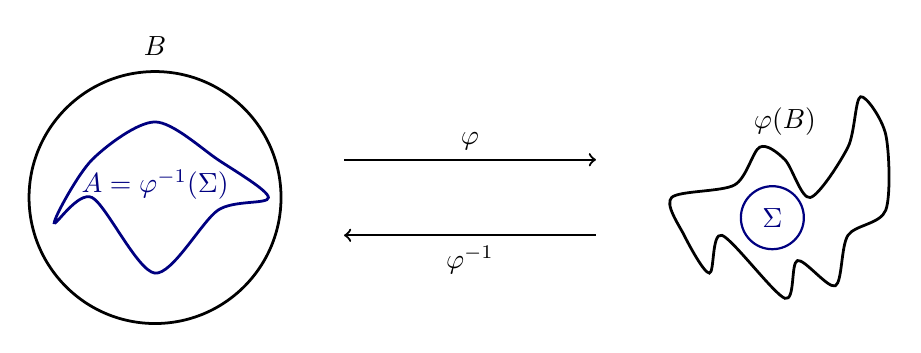
\begin{tikzpicture}[scale=1.6]
    \draw[thick,->] (-1,0.3)-- (1,0.3)%
    node[midway,above] {$\vphi$};
    \draw[thick,->] (1,-0.3) -- (-1,-0.3)%
    node[midway,below] {$\vphi^{-1}$}; 
    \draw[line width=1, black] (-2.5,0) circle (1);
    \draw node at (-2.5,1.2) {\color{black} $B$};
    \draw[line width=1, black] plot [smooth cycle, tension=0.5]%
    coordinates { (2.5,-0.8) (2.6,-0.5) (2.9,-0.7) (3,-0.3) (3.3,-0.1)% 
    (3.3,0.5) (3.1,0.8) (3,0.4) (2.7,0) (2.5,0.3) (2.3,0.4)%
    (2.1,0.1) (1.6,0) (1.7,-0.3) (1.9, -0.6) (2,-0.3)};
    \draw node at (2.5,0.6) {\color{black} $\vphi(B)$};

    \draw[thick, NavyBlue] (2.4,-0.16) circle (0.25);
    \draw node at (2.4,-0.16) {\color{NavyBlue} $\Sigma$};
    \draw[line width=1, NavyBlue] plot [smooth cycle, tension=0.5]%
    coordinates { (-2.5,-0.6) (-3, 0) (-3.3,-0.2) (-3,0.3) (-2.5,0.6)%
    (-2,0.3) (-1.6,0) (-2,-0.1)};
    \draw node at (-2.5,0.1) {\color{NavyBlue} $A=\vphi^{-1}(\Sigma)$};
  \end{tikzpicture}
  \caption{The construction of regions $A$, $B$, and $\hat{A}$ in the
  proof of Theorem~\ref{thm:dpp}.} 
\end{figure}

\begin{proof}
  Let $\varphi$ be a map projection, and let 
  $\kappa \subset U$ be some cap. We will take our regions 
  $A$ and $B$ to lie in $\kappa$. Set $B$ to be a cap 
  contained in $\kappa$. Let $\Sigma$ be a circle in 
  the plane such that $\Sigma
  \subsetneq \varphi(B)$ and let $A=\varphi^{-1}(\Sigma)$ (see
  Figure~\ref{fig:dpp}).

  We now use the isoperimetric inequality for the sphere 
  and Corollary~\ref{cor:capscale} to claim that 
  $A$ does not maximilze Polsby-Popper score in the sphere.

  To see this, take $\hat{A}$ to be a cap in the sphere with 
  area equal to that of $A$. Note that since the 
  area of $\hat {A}$ is less than the area of the cap $B$, it 
  follows that we can choose $\hat{A}\subset B$. 
  
  By the isoperimetric inequality of the sphere, 
  $\mathrm{PP}_S(\hat{A})\geq
  \mathrm{PP}_S(A)$. Since map projections preserve containment,
  $\Sigma\subsetneq \varphi(B)$ implies that $A\subsetneq B$, 
  meaning that $\mathrm{area}(\hat A) = \mathrm{area}(A)\lneq 
  \mathrm{area}(B)$. By Corollary~\ref{cor:capscale}, we know that
  $\mathrm{PP_S}(\hat{A})< \mathrm{PP_S}(B)$, and combining this with
  the earlier inequality, we get
  \begin{align*}
    \mathrm{PP_S}({A})\leq \mathrm{PP_S}(\hat{A})< \mathrm{PP_S}(B)
  \end{align*}

  Since $\Sigma = \varphi(A)$ maximizes the Polsby-Popper score in the
  plane, but $A$ does not do so in the sphere, we have shown that
  $\varphi$ does not preserve the maximal elements in the score
  ordering, and therefore it cannot preserve the ordering itself.
\end{proof}

The reason why every map projection fails to preserve the ordering of
Polsby-Popper scores is because the score itself is constructed from
the \textit{planar} notion of isoperimetry, and there is no reason to
expect this formula to move nicely back and forth between the sphere
and the plane.  This proof crucially exploits a scale invariance
present in the plane but not the sphere.  If we consider any circle in
the plane, it's Polsby-Popper score is definitionally equal to one,
but that is not true of every cap in the sphere.  \mute{This naturally
raises the question of whether being more careful, and defining
a compactness score which uses the isoperimetric quotient of the
surface the region is actually in will evade this problem.  We show
later that it does resolve the issue of scale-noninvariance, but it is
still induces an ordering which is not preserved by any map
projection.  We discuss this further in \Cref{sec:generalz}.}

\section{Isoperimetric Quotient}\label{sec:isoper}


We remarked at the end of Section~\ref{sec:pp} that a more principled version of an isoperimetric quotient may avoid the failure of the ordinary Polsby-Popper score to induce an ordering which can be preserved by some map projection.

\begin{definition}
We define the \textbf{isoperimetric quotient score} of a region $\Omega$ to be$$
\mathrm{IPQ}(\Omega)=
\begin{cases}
\frac{4\pi \ \mathrm{area}(\Omega)}{\mathrm{perim}(\Omega)^2} \text{ in the plane},\\[10pt]
\frac{\mathrm{area}(\Omega)^2 - 4\pi \ \mathrm{area}(\Omega)}{\mathrm{perim}(\Omega)^2}\text{ on the sphere}
\end{cases}
$$
\end{definition}

This score properly resolves the issue of scale-noninvariance, and the isoperimetric quotient scores of circles in the plane \textit{and} caps on the sphere are one, regardless of their size.

We'll prove order non-preservation in the same way as before, and we built all of the machinery needed to do it in the previous section.  Since any order-preserving map projection needs to preserve the maximizers and caps and circles maximize the isoperimetric quotient score, we can restrict our attention to map projections which send caps to circles.  We showed in the previous section that these are exactly the projections which are the composition of the stereographic projection and a scaled isometry of the plane.  Since this score is scale-invariant, it is preserved by scaled isometries, so we only need to demonstrate the existence of regions on the sphere whose scores are permuted by the stereographic projection.


\begin{theorem}
There exist two regions on the sphere $A$ and $B$ such that $\mathrm{IPQ}(A)>\mathrm{IPQ}(B)$ but under the stereographic projection $\varphi$, $\mathrm{IPQ}(\varphi(A)))<\mathrm{IPQ}(\varphi(B))$.
\end{theorem}



\begin{proof}
Using the same construction as in the proof of Theorem~\ref{thm:reock}, since the image under the stereographic projection of $\kappa'_N$ has both smaller area and larger perimeter than the image of $\kappa'_S$, the isoperimetric quotient score of the image of $\kappa'_N$ in the plane is strictly worse than the score of the image of $\kappa'_S$, although they have the same score as regions on the surface of the sphere.

\end{proof}


The remainder of the argument also follows from our previous results.  Lemma~\ref{lem:noafflin} says that no scaled isometry can correct for the permutation of score ordering, so there does not exist a map projection which preserves the ordering over regions induced by the isoperimetric quotient score.








\section{Empirical Results}\label{sec:exper}




While we have shown mathematically that the ordering of compactness scores can be permuted by any map 
projection, the actual districts we wish to examine are relatively small compared to the surface of the Earth, 
and we might ask whether this order reversal actually occurs in practice.
We can extract the boundaries of the districts from a \textit{shapefile} from the U.S. Census Bureau\footnote{We use the U.S. Census Bureau's shapefile for the Congressional districts for the 115th Congress.} and compute the convex hull, Reock, and Polsby-Popper scores on the Earth and with respect to a common map projection\footnote{The code to compute the various compactness scores is based on Lee Hachadoorian's \textit{compactr} project \cite{hachadoorian2018reock}.} and examine the ordering of the districts with respect to both.

The projection we use is the familiar \textit{Mercator} projection, which is commonly used in settings like Internet mapping applications and pulldown maps in school classrooms.  The Mercator projection presents latitudes and longitudes as equally-spaced horizontal and vertical lines, which causes small amounts of distortion near the equator, but large amounts outside of the tropics, with the areas of regions near the poles being dramatically inflated under the projection.








We observe overall that the orderings of under the Polsby-Popper score and convex hull score are relatively undisturbed compared to that of the Reock score.  This is because the \textit{values} of those scores do not change by too much under different projections.  Intuitively, this is because while both projections distort shapes, they do so in a way that does not affect either of these scores by too much, since in the case of the Polsby-Popper score, the perimeter and area of the regions are changed in similar ways, and in the case of the convex hull score, the area of the convex hull of a region is distorted in the same way as the region itself, so the ratio of the areas is similar across projections.

For regions in North America, such as our Congressional districts, the differences in the minimal bounding circle between the spherical and Mercator representation cause massive differences in both the raw values of the scores as well as the ordering.  The scores can change in either direction by upwards of $.1$ (recall that the value of the score is between zero and one) and there is almost no correlation in the ordering of the districts by their Reock scores on the sphere and under the Mercator projection. 



\section{Conclusion and Future Directions}\label{sec:future}
We demonstrate here the failure of a standard panel of compactness measures to provide a consistent score ordering over all regions.  
While compactness scores are not used critically in a \textit{legal} context, they appear frequently in the popular discourse about redistricting issues and frame the perception of the `fairness' of a plan.  For example, a 2014 Washington Post piece  \cite{ingraham2014solve} describes an algorithm which generates highly compact districts because it ignores all of the social and demographic data which are crucial to the process.  The equating of `solving' gerrymandering with generating highly compact districts presupposes that the mathematics used to evaluate the geometric features of districts are unbiased and unmanipulable, and we demonstrate here that this is certainly not the case.


The results here suggest that more nuanced models of compactness are worth exploring.  Graph-theoretic (i.e. `discrete') compactness measures as in \cite{deford2018tv,duchin2018discrete} are computed without reference to any particular metric embedding, so they definitionally cannot be affected by the choice of map projection.  Multiscale measures of compactness as in \cite{deford2018tv} provide a higher resolution view of the geometry of regions.  The authors there leave open the question of to what degree a region's total variation profile is unique, and a strongly positive result to that problem would suggest that you can't ``hide'' any of the geometry of a region using the choice of map projection.

This work opens several promising avenues for further investigation.  We prove strong results for the most common compactness scores, but the question remains what the most general mathematical result in this domain might be, such as giving a set of necessary and sufficient conditions for a compactness score to not induce a permuted order for some choice of map projection.  Generalizing these results to other surfaces and non-standard measures (such as weighting by population) may also be an avenue for examination.


\bibliographystyle{plainnat}
\bibliography{bib.bib}

\end{document}
